% !TeX root = ../../../book.tex
\section{定义与示例}

你通常是如何看待一个函数的?对函数的直观理解是什么?你会如何用数学对象来\emph{定义}函数呢?你以前尝试过这样定义函数吗?试试看吧!想想我们已经学过的概念和工具,能不能仅用这些概念来表达你对\emph{函数}的理解呢?认真试一下!先阅读接下来的几段内容,我们会逐步建立函数的定义,然后你再尝试自己给出一个定义。

我们通常认为函数是一种\emph{规则}或\emph{映射},用来告诉我们如何将输出值分配给任意给定的输入值。例如,定义在 $\mathbb{R}$ 上的函数 $f(x) = x^2$,它接受一个实数作为输入并输出该实数的平方。函数 $f$ 就像一台``机器'',把一个数字变成它的平方;说函数``在 $\mathbb{R}$ 上''意味着我们只能把实数放进这台机器。那么,我们怎么知道机器允许输出什么呢?我们已经发现了对函数解释中的一个缺陷。理想情况下,我们希望在定义函数时传达所有必要的信息:输入可以是什么,输出可以是什么(不一定是所有可能的输出,也可以是什么类型的对象),以及``规则''是什么。如果你把函数看作一个\emph{映射},那么它就像是描述如何通过某种集合间的``道路''(在这个例子中是取输入数的平方),从一组数字(在这种情况下是 $\mathbb{R}$)导航到另一组数字(也是 $\mathbb{R}$)。在这种解释中,我们仍然希望传达刚才提到的所有信息,但也指出了其他的理解方式。

在我们给出定义之前,先来思考一个问题。假设有一个``规则'',它的输入是一个人,而输出是这个人的眼睛颜色。你会如何将其表示为 $f(x) = \dots$ 的形式呢?这很难!你几乎需要将前一句话完整地重写,才能定义这个``规则''。那么,允许的输入和输出是什么呢?它们既不是实数也不是整数,而是完全不同的东西。然而,这个函数是合理的,我们希望在定义中包含它。思考一下这种情况与 $f(x) = x^2$ 在实数集 $\mathbb{R}$ 上的函数有何不同(或者实际上并没有什么不同)。(你甚至可能会反对说这根本就不是一个\emph{函数}!万一一个人有两种不同颜色的眼睛呢?这个``映射''的输出又是什么呢?哦,天哪!)

好了,现在轮到你了。试着用我们在前几章讨论过的概念、术语和数学对象来定义\emph{函数}。

% !TeX root = ../../../book.tex

\subsection{定义}

我们将使用以下定义。或许它与你的定义接近,甚至相同,或者只是措辞略有不同。但这个定义完美地概括了我们前面对函数的直观概念(将函数看作一种分配\emph{规则}),并用我们一直以来在发展的集合和逻辑语言来表达。这样做有几个好处:

\begin{enumerate}[label=(\alph*)]
    \item 它为函数提供了严格的基础,使我们能够在数学意义上放心地使用它们;
    \item 它让我们能够讨论函数的性质,并用数学术语和概念来证明这些性质;
    \item 它使我们能够概括函数的概念,并将其应用于比我们熟悉的标准数集更抽象的场景中。
\end{enumerate}
好了,解释到此为止,我们来看定义。\\

\begin{definition}
    设 $A, B$ 为集合。设 $f$ 为 $A, B$ 间的关系,所以 $f \subseteq A \times B$。同时假设 $f$ 具有如下性质:
    \[\forall a \in A \centerdot \exists! b \in B \centerdot (a, b) \in f\]
    (回想一下,``$\exists!$'' 表示``存在唯一的……'',也就是说``有且只有一个……'')

    这样的关系称为 $A$ 到 $B$ 的 \dotuline{函数}。

    我们称 $A$ 为函数的\dotuline{定义域},$B$ 为函数的\dotuline{值域}。

    写做
    \[f:A \to B\]
    表示 $f$ 是 $A$ 到 $B$ 的函数。

    如果 $(a,b) \in f$,则我们写做
    \[f(a) = b\]
    并且知道对于给定的 $a$,$b$ 是唯一满足该属性的元素。
\end{definition}

就是这样!虽然现在把\emph{函数}看作一种\emph{关系} --- 实际上是一种特殊的\emph{集合} --- 可能有点奇怪,但这正是它的本质。用这种方式定义函数让我们能够用集合和关系的语言来讨论它们,同时我们仍然可以使用一些熟悉的符号。对于每一个``输入'' $a$(即\emph{定义域}中的每一个元素),都有\emph{唯一}一个``输出'' $b$(即\emph{值域}中的一个元素)。因此,我们可以写成 $f(a) = b$,并且知道 ``$=$'' 表示真正的相等关系,因为只有这个唯一的 $b$ 满足这种关系。

这种定义的一部分包含了我们之前提到的想法:我们想知道函数会``输出''什么\emph{类型}的对象。这就是通过指定值域实现的。例如,定义函数 $f : \mathbb{R} \to \mathbb{R}$ 为 $f(x) = \sqrt{x}$ 是不合适的,因为定义域中的某些元素(即负数)会使``输出''未定义。(技术上讲,输出会是一个复数,而复数不是值域 $\mathbb{R}$ 的元素;在 $\mathbb{R}$ 的上下文中,我们认为复数是``未定义''的。)当一个函数被正确定义,且定义域和值域已明确,并且相关的对确实属于集合的笛卡尔积时,我们称这个函数是\textbf{良好定义的}。有时,我们会给出两个集合之间的关系,并要求你判断它是否是\emph{良好定义的函数}。实际上,这就是在问这个关系是否符合函数的定义。

\subsubsection*{范围}

\emph{值域}这个词对你来说可能比较陌生。实际上,你可能更习惯用\textbf{范围}来指代函数的\emph{潜在}``输出''集合。我们想在这个上下文中完全避免使用``范围''一词,因为它可能会产生歧义。有些作者和老师用``范围''来表示我们这里所说的``值域'',即函数的\emph{潜在}``输出''集合;而另一些人则用它来表示本书所说的``像'',即函数的\emph{实际}``输出''集合。在 \ref{sec:section7.3} 节中我们会详细定义这个术语。通常,像是值域的子集,但往往可能是\emph{真}子集。当有人使用``范围''这个词时,他们可能指的是这两种解释中的其中一个,而你可能理解的是另一个!为了避免这种混淆,我们将只使用\emph{值域}和\emph{像}这两个词。

% !TeX root = ../../../book.tex

\subsection{示例}

让我们使用新的定义来看几个函数(以及非函数)的例子。在处理这些例子时,我们将介绍定义和使用函数的正确符号,并描述如何``可视化''某些函数,以便更好地理解它们。

\subsubsection*{符号}

有几种正确定义函数的方法。以下都是定义``实数平方函数''的正确方法:
\begin{quotation}
    定义函数 $f \subseteq \mathbb{R} \times \mathbb{R}$ 为 $(x, y) \in f \iff y = x^2$。

    定义函数 $f : \mathbb{R} \to \mathbb{R}$ 为 $f=\big\{(x,x^2) \mid x \in \mathbb{R}\big\}$。

    定义函数 $f : \mathbb{R} \to \mathbb{R}$ 为 $\forall x \in \mathbb{R} \centerdot f(x) = x^2$。
\end{quotation}
考虑每种方法为什么符合我们上面给出的函数定义。第一种方法直接表明函数是一种\emph{集合},即从 $\mathbb{R}$ 到 $\mathbb{R}$ 的关系。第二种方法使用相同的概念,但通过集合构建符来表示 $f$,而不是用\emph{充要条件}语句。第三种方法表明每个 $f$ 的``输入''都有\emph{唯一}一个``输出'',所以我们可以简单地声明\emph{对于所有} $x \in \mathbb{R}$ 的``输出''。

我们\emph{通常}会坚持使用第三种符号风格,因为它更容易理解,并且更符合我们对函数的直观认识。有时,我们也会使用其他符号风格;例如,我们想要强调函数的底层结构,或者仅仅可能是为了更容易书写。不过,一般来说,在定义函数时,我们需要为读者明确所有重要的组成部分:\emph{定义域}、\emph{值域}、\emph{函数名},以及分配有序对的\emph{规则}或\emph{集合}。

如果你在想为什么在定义函数时指定\emph{值域}如此重要,可以从编写计算机代码的角度来考虑。当你定义一个函数时,通常需要\emph{声明}输出变量的数据类型。(当然,这也取决于具体的编程语言。)以 \verb|Java| 为例,你可能会写
\begin{verbatim}
    public int PlusOne (int x) {
        return x+1;
    }
\end{verbatim}
上面代码定义了一个函数,它输入一个整数,加一后输出另一个整数。请注意,你必须告诉程序输入的数据类型是什么以及输出的数据类型是什么。\\

\begin{example}
    考虑一个将自然数转换为其二进制表示的函数。我们用 $B$ 表示这个函数。通过计算,我们希望 $B(1) = 1, B(2) = 10, B(10) = 1010$。那么,这个函数的定义域是什么?值域是什么?你能严格地写出它的定义\emph{规则}吗?还是用文字描述更好呢?

    我们可以这样定义这个函数。设 $S$ 为所有由 $0$ 和 $1$ 组成的有限二进制字符串的集合。然后定义函数 $B : \mathbb{N} \to S$ 为
    \[B = \{(n, s) \mid n \in \mathbb{N} \;\text{且}\; s \;\text{为}\; n \;\text{的二进制表示}\}\]
\end{example}

\begin{example}
    再次考虑``平方函数'':设 $f : \mathbb{R} \to \mathbb{R}$ 定义为 $\forall x \in \mathbb{R}, f(x) = x^2$。这函数与下面的函数有区别吗?
    \begin{itemize}
        \item 设函数 $g : \mathbb{R} \to \mathbb{C}$ 定义为
            \[\forall x \in \mathbb{R} \centerdot g(x) = x^2\]
        \item 设函数 $h : \mathbb{Z} \to \mathbb{R}$ 定义为
            \[\forall x \in \mathbb{Z} \centerdot h(x) = x^2\]
    \end{itemize}

    函数 $g$ 的值域不同,但实际上,$\mathbb{R} \subseteq \mathbb{C}$。所有有序对 $(x, x^2) \in g$ 仍然满足 $x \in \mathbb{R}$ 且 $x^2 \in \mathbb{R}$。从这个角度来看,$f$ 和 $g$ 是\emph{相同的}函数,我们可以写做 $f = g$。稍后,我们将详细探讨两个函数相等的确切含义。目前,只需说明 $f$ 和 $g$ 对应的底层关系具有相同的实数有序对作为元素即可。理论上,函数 $g$ \emph{允许}第二个值为复数,但由于定义域和``规则''的设定,这实际上不会发生。

    函数 $h$ 的定义域不同,并且 $\mathbb{Z} \subset \mathbb{R}$(是 $\mathbb{R}$ 的真子集)。因此,在函数 $f$ 对应的关系中,有许多有序对并不属于函数 $h$ 对应的关系。例如,$(\frac{1}{2}, \frac{1}{4}) \in f$ 但 $(\frac{1}{2}, \frac{1}{4}) \notin h$。换句话说,$f(\frac{1}{2}) = \frac{1}{4}$,但 $h(\frac{1}{2})$ 的概念没有\emph{良好定义},因为 $\frac{1}{2}$ 不属于 $h$ 的定义域。
\end{example}

\begin{example}
    我们也可以\textbf{分段}定义函数。例如,考虑定义在 $\mathbb{R}$ 上的\emph{绝对值函数}:

    设函数 $a : \mathbb{R} \to \mathbb{R}$ 定义为
    \[\forall x \in \mathbb{R} \centerdot a(x) = 
    \begin{cases}
         x &\text{如果}\; x \ge 0 \\
        -x &\text{如果}\; x < 0
     \end{cases}\]
     定义域中的每个元素都\emph{恰好}落入某一种情况,因此没有歧义。
\end{example}

\subsubsection*{``良好定义的''函数}

我们并不总是能明确一个定义的关系是否真正是一个函数。面对一个给定的定义域、值域和一个``规则''或集合,我们该如何验证它们是否构成一个函数呢?接下来我们将给出一个定义(完全基于之前讨论的函数定义)来解决这个问题:

\begin{definition}\label{def:definition7.2.5}
    给定定义域 $A$、值域 $B$ 和``规则'' $f$,我们说 $f$ 是一个\dotuline{良好定义的函数},当且仅当
    \begin{enumerate}[label=(\arabic*)]
        \item 该规则定义在 $A$ 的所有元素上;
        \item 对于每个 $a \in A$,该规则都输出集合 $B$ 中的唯一一个元素。
    \end{enumerate}
\end{definition}

让我们用一个例子来说明这个概念。在本节的后面,我们还会看到一些不是函数的例子,并且会再次引用这个\textbf{良好定义的函数}的定义。\\

\begin{example}
    设函数 $a : \mathbb{Z} \to \mathbb{N}$ 定义为
    \[\forall z \in \mathbb{Z} \centerdot f(z) = |2z + 1|\]
    等一下,我们怎么确定对于任意\emph{整数} $z$,$|2z + 1|$ 为\emph{自然数}?这不是那么显然,但我们可以证明出来。

    假设 $z \in \mathbb{Z}$ 满足 $z \ge 1$。则 $2z+1 \in \mathbb{Z}$ 且 $|2z+1| = 2z+1 \ge 3$。因此 $f(x) \in \mathbb{N}$。

    假设 $z \in \mathbb{Z}$ 满足 $z \le -1$。则 $2z+1 \in \mathbb{Z}$ 且 $2z+1 \le -1$。因此 $f(x) = |2z + 1| ≥ 1 \in \mathbb{N}$。所以 $f(x) \in \mathbb{N}$。

    假设 $z = 0$。则 $f(z) = |2 \cdot 0 + 1| = 1$,所以 $f(z) \in \mathbb{N}$。

    无论哪种情况,我们发现定义函数 $f$ 的``规则''确实会生成一个自然数,这个数是\emph{值域}中的元素。而且,它只生成这样一个数。因此,这是一个良好定义的函数。
\end{example}

\begin{example}
    设 $P$ 为世上所有人的集合。函数 $b : P \to \mathbb{N} \cup \{0\}$ 定义为
    \[b = \{(p, n) \mid p \in P \land p \;\text{有}\; n ;\text{个姐妹}\}\]
    (请注意,为了练习,我们这里使用了一种强调集合的符号风格。另外,将数学符号和文字结合起来可能看起来有些奇怪,例如 ``$b(p) = p \;\text{这个人有多少个姐妹}$''。)

    这是一个良好定义的函数吗?我们认为是的。假如你走到某人面前(即某个元素 $p \in P$),问他们有多少姐妹(即 $b(p)$ 的值)。他们会告诉你一个非负整数,并且他们不可能给出两个\emph{不同的}数字。

    现在,你可能会指出,在今天这个离婚和再婚普遍的社会中,很多人有\emph{同父异母或同母异父的姐妹} (half-sisters),而 $\frac{1}{2} \notin \mathbb{N} \cup \{0\}$。这个观点很合理。但是,在``简化假设''下,即假设每个人都有\emph{整数数量}的姐妹,这个函数是良好定义的。
\end{example}

\subsubsection*{恒等函数}

\begin{example}
    设 $S$ 为集合。是否\emph{必然}存在一个从 $S$ 到 $S$ 的函数?当然,我们可以想到许多从 $\mathbb{R}$ 到 $\mathbb{R}$ 的函数,但如果 $S$ 只是某个任意集合呢?我们能保证存在一个从 $S$ 到 $S$ 的函数吗?事实证明……是的,我们可以!回想一下我们在讨论关系时曾考虑过的一个类似问题(参见示例 \ref{ex:example6.2.9})。我们知道在集合 $S$ 上我们总是可以定义\emph{等价关系};也就是说,我们可以通过 $(x, y) \in R \iff x = y$ 在 $S$ 上定义 $R$。对于每个 $x \in S$,这个关系由所有形式为 $(x, x)$ 的有序对组成。这个关系是否表示一个函数?我们只需检查定义属性:每个输入是否只有一个输出?看起来确实如此!集合中的任意元素只等于它自己,而不等于其他任何元素。因此,$R$ 确实表示一个函数。这是一个特别的函数,我们给它起了一个特定的名字。
\end{example}

\begin{definition}
    设 $S$ 为集合。$S$ 上的\dotuline{恒等函数}为函数 $Id : S \to S$ 定义为
    \[\forall x \in S \centerdot Id(x) = x\]
\end{definition}

也就是说,恒等函数``输出与输入完全相同''。(可以把函数想象成一台机器,这台懒惰的机器什么也不做,只是原样输出输入的内容。)

有时,我们需要引用在\emph{不同}集合上定义的恒等函数。为避免混淆,我们用 $Id_S$ 表示``\textbf{集合 $S$ 上的}恒等函数''。

\subsubsection*{不是函数的例子}

有时候,在解决问题时,我们可能会提出一个关于两个集合之间的``规则'',并想知道它是否是一个函数。也许我们需要它是一个函数来帮助我们解决问题。那么,这个规则在什么情况下可能不成立呢?换句话说,我们可以通过什么来证明一个提出的规则不是一个函数呢?回顾一下\textbf{良好定义的函数}的定义(见定义 \ref{def:definition7.2.5}),有三种不同的情况可能出错:

\begin{itemize}
    \item 可能存在某个定义域中的元素\textbf{没有对应的``输出''}。
    \item 可能存在某个定义域中的元素\textbf{有多个``输出''}。
    \item 可能存在某个定义域中的元素只有一个``输出'',但该``输出''\textbf{不在值域中}。
\end{itemize}
以下例子说明了这些情况。\\

\begin{example}
    设函数 $G : \mathbb{N} \times \mathbb{N} \to \mathbb{N}$ 定义为
    \[\forall (a, b) \in \mathbb{N} \times \mathbb{N} \centerdot G(a, b) = a - b\]
    这\textbf{不是}一个良好定义的函数,因为有定义域中的很多元素其输出不在值域中。例如,$(5, 10) \in \mathbb{N} \times \mathbb{N}$ 且 $G(5, 10) = -5$,但 $-5 \notin \mathbb{N}$。
\end{example}

\begin{example}
    假设 $W$ 为所有英语单词的集合。定义 $A: W \to W$ 为输入一个单词并输出一个不是原单词的变位词。这\textbf{不是一个良好定义的}函数,原因有几个。例如,$A(\text{HI})$ 和 $A(\text{FUNCTION})$ 都不存在。此外,像 $A(\text{INTEGRAL})$ 这样的单词有多个(即非唯一的)输出:TRIANGLE, ALERTING, ALTERING……。
\end{example}

% !TeX root = ../../../book.tex

\subsection{函数相等}

% !TeX root = ../../../book.tex

\subsection{示意图}

在我们深入讨论函数的抽象性质及其证明方法之前,我们先介绍一种有助于表示函数的方法。需要强调的是,这种方法在数学上并不\emph{严谨},在\emph{证明}中使用可能不是最佳选择。(例如,在评分的作业中,即使你有正确的想法,可能也不会得满分。)然而,这种方法确实能直观地展示函数的工作原理,并帮助你发现问题并进行更严格的证明。特别是,这种方法在构造函数性质的\emph{反例}时非常有用。

\textbf{示意图}的概念类似于我们用\emph{韦恩图}表示集合。集合是元素的集合,而不是纸上的阴影圆圈,但这些阴影圆圈及其重叠可以帮助我们理解和描述集合。同样,函数是两个集合之间具有特定属性的关系,而不是像这样:

\begin{center}
    {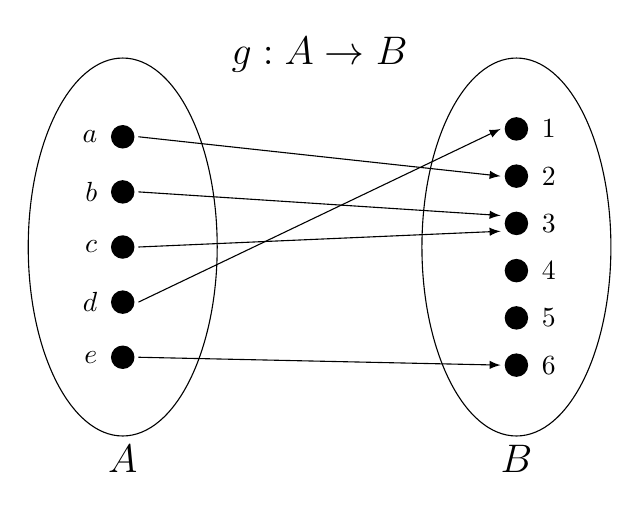
\begin{tikzpicture}[scale=1]
        \foreach \x in  {1,...,6}
        {
            \node at (5, -\x*0.6)[circle,fill,inner sep=3pt]{};
            \draw[shift={(5.2, -\x*0.6)}] node[right] {$\x$};
        }
        \draw (5,-2.1) ellipse (1.2 and 2.4);

        \foreach \x/\s in  {1/a,2/b,3/c,4/d,5/e}
        {
            \node at (0, -\x*0.7)[circle,fill,inner sep=3pt]{};
            \draw[shift={(-0.2, -\x*0.7)}] node[left] {$\s$};
        }
        \draw (0,-2.1) ellipse (1.2 and 2.4);

        \draw[-latex] (0.2,-0.7) -- (4.8,-1.2); 
        \draw[-latex] (0.2,-1.4) -- (4.8,-1.7); 
        \draw[-latex] (0.2,-2.1) -- (4.8,-1.9); 
        \draw[-latex] (0.2,-2.8) -- (4.8,-0.6); 
        \draw[-latex] (0.2,-3.5) -- (4.8,-3.6);
        
        \node[below] at (0, -4.5){\Large $A$};
        \node[below] at (5, -4.5){\Large $B$};
        \node[above] at (2.5, 0){\Large $g:A \to B$};
    \end{tikzpicture}}
\end{center}

然而,这在某种程度上确实\emph{代表}了函数的概念。在这幅图中,我们用椭圆分别表示了定义域 $A$ 和值域 $B$。$A$ 和 $B$ 的元素则用椭圆内的点来表示,并且进行了标记。我们根据函数 $g: A \to B$ 在这些点之间画上箭头。

这种方法通常用于探索函数的特性,或者构造反例来反驳某个主张。通过绘制一些点和箭头,并尝试它们的连接方式,我们可以逐步构建一个例子的基础\emph{结构}。然后,再为图中的各部分分配名称和公式,使其更加严谨。

在我们的讨论中,我们会用一些示意图来说明某些属性和概念,同时提供更严谨的陈述或描述。我们鼓励你也采用这种方法。

% !TeX root = ../../../book.tex

\subsection{习题}